\label{sec:queries}

\subsection{Slicing An Image Cube}

Now that the data has been ingested into Rasdaman we proceeded with writing simple queries. Since Rasdaman is an Array Database system which has been used for multi-dimensional data we first wanted to start this part of the project by reproducing the functionaility of the ATLAS viewer described above. For this we want to start with simple slicing operations, namely just extracting Sagittal, Coronal and Axial\footnote{Sagittal, Coronal and Axial cuts are domain specific terms for cuts parallel to the axes of the data cube. } slices from the original scan.

Rasdaman is capable of expressing these cuts easily. Each of them is parameterized by two parameters, the two axes it is parallel to and the position within the third axis where to cut. In the query language this uses a slicing operation and is written as \lstinline[morekeywords={NAME,INDEX},language=SQL]{select it[INDEX,*:*,*:*] from NAME as it}. Here \lstinline{INDEX} refers to the position of where to cut and \lstinline{NAME} refers to the name of the collection that contains the data cube.

\begin{figure}[h]
\centering
\begin{subfigure}{.3\textwidth}
  \centering
  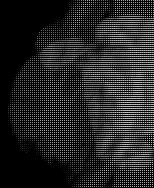
\includegraphics[width=\textwidth]{imgs/CutA}
\end{subfigure}%
\space\space\space
\begin{subfigure}{.3\textwidth}
  \centering
  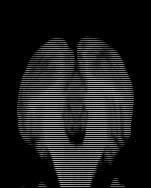
\includegraphics[width=\textwidth]{imgs/CutB}
\end{subfigure}
\space\space\space
\begin{subfigure}{.3\textwidth}
  \centering
  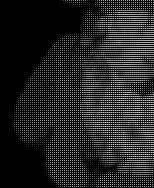
\includegraphics[width=\textwidth]{imgs/CutC}
\end{subfigure}
\caption{Simple cuts through the example dataset. }
\label{fig:cuts}
\end{figure}

Additionally in order to display the output from this operation we need to choose an image format to display it in. To save such a cut as a png image a command like
\begin{lstlisting}[showstringspaces=false,morekeywords={NAME,INDEX,FILENAME},language=Bash]
rasql -q "select encode(it[INDEX,*:*,*:*],\"png\") from NAME as it" --out file --outfile FILENAME
\end{lstlisting}
can be used. A sample output of this operation can be found in Figure~\ref{fig:cuts}.

\subsection{Overlaying Brain Region Masks}

The second operation of the ATLAS viewer that is interesting to reproduce is the overlaying of Brain Region Masks onto the original scan. This operation is more complicated than the simple slicing operation and any query performing it needs to perform the following three steps:
\begin{enumerate}
  \item retrieve the brain scan data
  \item retrieve the brain mask data
  \item overlay the mask over the brain data
\end{enumerate}

A command similar to the following could be used to produce a single Brain region mask overlay:
\begin{lstlisting}[showstringspaces=false,morekeywords={INDEX,MASK_COLLECTION,SCAN_COLLECTION,FILENAME},language=Bash]
rasql -q "select encode(S[INDEX,*:*,*:*] overlay M[INDEX,*:*,*:*], \"png\") from MASK_COLLECTION M, SCAN_COLLECTION S" --out file --filename FILENAME
\end{lstlisting}

In this command we assume that the brain scan data and the mask data are available in the collections \lstinline{SCAN_COLLECTION} and \lstinline{MASK_COLLECTION} respctively. Then we use the \lstinline{overlay} operator to overlay the two images.

\begin{figure}[h]
  \centering
  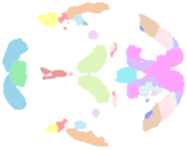
\includegraphics{imgs/Mask}
  \caption{Example Brain Mask Data}
  \label{fig:mask}
\end{figure}

In practive the second step of retrieve brain mask data provides significant difficulties. Even though the brain mask data is available in principal it is only given in the form of an SVG image. Unlike the brain scan data, this is a vector image format which does not store the rasterized representation as would be needed by Rasdaman. On top of this the SVG images do not contain three-dimensional data but are instead structured similar to the BBIC format. For each possible cut and zoom level a seperate image is provided. One of these image can be found in Figure~\ref{fig:mask}. Unfortunatly these problems stopped us from properly ingesting the brain mask data into Rasdaman.

\subsection{Extended Slices}

The final type of query we wanted to experiment with expands on the slicing explained above. Instead of only allowing cuts parallel to two of the three axes we wanted to allow any type of two-dimensional cuts. While this is not available in the ATLAS viewer it is an enhancement our collaborators have been thinking about. Mathematically speaking such a cut consists of an arbitrary two-dimensional plane intersecting a three-dimensional cuboid. As such it is parametrised by 6 parameters, one (three-dimensional) point to start the plane at and three angles in each direction to rotate the plane along.

This mathematical description gives us one natural way to represent this query inside Rasdaman: Rotate the entire cube according to the three angles given above and then perform a simple cut as described above. Unfortunatly there is no rotation operation inside Rasdaman, but according to \cite{rasdaman:issue228} it might be added in the future.

There is a second way to represent these queries inside Rasdaman. Outside of Rasdaman one can compute the coordinates that would be included in the plane and then query the database for those exact values. Even though this could be simplified by using arrays to index the data cube, this still requires some non-trivial computational effort outside of Rasdaman and thus we did not perform this query either.
